\chapter{Introduction\label{cha:introduction}}

In the late 19th century a Germand student named Paul Gottlieb Nipkow developed an electronical device
that was able to send images over the wire with the help of a rotating metal disk. This was one of the first
mechanical prototypes that suppose to become the television. With the beginning of the 20th century two types
of TVs emerged: mechanical and electronic television. Even though the mechanical type has seen a lot of
innovation by 1934, all television systems had been converted to electronic machines. These became more and
more popular in humans households so that almost 10 years later the number of U.S. homes with television sets
could be measured in the thousands and by the late 1990s more than 98\% of U.S. homes had at least one
television. The device was one of the first electronic devices that introduced a new generation of entertainment
human equiment that everyone suppose to have.\\
Despites innovations like colored displays or flat screen devices the television quickly lost the race against
the mobile phone as well as the personal computer and later laptop. Even though it is still a very popular
medium, people nowadays use their smart phone or personal computer way more frequent as it was at the end of the
20th century. One of the major reasons was the innovation of the internet. The more people were able to connect
each other and consum media over the world wide web the more became the television the less frequent choice.
The new generation of kids grows up with web media portals like YouTube\footnote{\url{https://www.youtube.com/}}
and generates billions and billions of clicks, views and revenue for advertisment companies every day.\\
Thanks to the most recent big innovations in television technology that are setup boxes and standards like
Hybrid Broadcast Broadband (short for HbbTV) the TV industries tries to keep up with other technologies by
introducing the so called smart televisions or sometimes referred to as connected TV or hybrid televisions.
It is the first generation of such devices that are connected to the world wide web and therefor can provide
digital content in a non linear way for the first time.\\
Since then the market and the amount of smart TVs has been growing fast. With that the HbbTV standared evolved
and more and more broadcaster have build an app for their broadcast streams. World wide have more than 25
countries (mainly in Europe) adopted the standard and broadcaster have developed around 300 apps that can
be viewed by more than 43 million sold devices with HbbTV support\footnote{\url{https://www.hbbtv.org/news-events/hbbtv-ibc-2016-services-and-devices/}}.
Numbers are growing. It shows the tremendous potential of the market and the beginning of a paradigm shift
from linear TV stream to non linear media content ondemand.

\section{Motivation\label{sec:motivation}}

By introducing TVs to the Internet it automatically opened the door for web technologies to become standards
on these devices. While early setup boxes like Chromecast\footnote{\url{https://www.google.com/intl/de_de/chromecast/}}
enabled some web-browsing experience, HbbTV has been the first real technology that brought websites to the big screen.
Instead of just watching a stream with linear content, HbbTV supported devices also provide web sources that
contextually fits to the viewed content and allow the user to navigate through an app to watch non linera content
ondemand.\\
These apps are webpages with JavaScript heavy functionality that are rendered in proparitary browsers. Unlike
normal browsers though there is no navigation menu or status bar. The page is rendered with a transparent background
so that you can show the TV stream in the back while navigating through the app. Depending on the TV manufacture
the embedded browser in the TV is mostly a clone to the existing desktop browsers though with less compatibility.
Early HbbTV supported devices are compatible with desktop browsers that have been shipped more than 10 years ago.
Especially since HbbTV runs a lot of JavaScript to show its content in a dynamic way this makes it hard for
developers to build their apps.\\
Compared to modern web development where almost everything is made out of web components, build together in a
modular fashion using tools like React, Polymer or Angular, HbbTV apps are still build like JavaScript single
page applications from 10 years ago. Not only because the technology within the browser doesn't allow to use
latest web technologies also the developer integration with common used tools on the developers machine is due
to device boundaries not possible. Since the internet is around way longer than the fact that it is supported on
TV devices the process of web development has become an own industry and tooling around it an own market.
Companies constantly build frameworks, tools and integrations that makes building complex web apps easier and
maintainable. Especially browser vendors like Google or Mozilla are interested in providing an excellent
developing experiences as this has become the only differentiator between browsers these days. After web
technologies has been standardised by the W3 Consortium\footnote{e.g. latest HTML specification: \url{https://www.w3.org/TR/html5/}}
the compatition between browsers is not based on the question who can interpret the HTML code better and therefor
render the page more correctly but more on which browser supports the latest recommended standards and fanciest
technologies.\\
Unfortunatelly this is not the case for all embedded browser in smart TVs. The HbbTV standard was developed as
a superset of HTML and JavaScript. The specification itself recommends support for certain APIs but doesn't
require the manufacture to embed the latest browser and all their features. This is partially due to the fact
that not all web technologies are applicable on a television. For example there is no WebRTC support because
most of the TVs don't have a camera installed. Also an HbbTV application was suppose to only add contextual
information to the provided broadcast stream. Building complex web applications was never considered to become
realitiy at the first place. However as more broadcaster discovered the opportunities that HbbTV can bring to
the audience more people were interested in finding new ways to deliver interactive content to everyone in
front of the screen.\\
This yields a problem that has been around in web development for ages but almost died due to the standardisation
of web technology. With more support for the HbbTV standard the manufacture started to improve the functionaility
of embedded browser not only by adding more computing power to smart TVs but also by providing better compatibility
to already accepted web standards. In addition to that the HbbTV standard itself evolved and requires now certain
technology to be supported in order to allow the TV to label itself as HbbTV compliant. The problem with this is
that not everyone buys a new TV as soon as there is a better one on the market. Especially since they last longer
than usual mobile phones or computer the update cycles of televisions are long. Compared to desktop browser which
update themself automatically and have reached version numbers in the fifties, the browser within todays smart
TVs don't update and stick as long as the owner keeps the television. This creates a highly fragmented
user market with tons of different devices over time that all support a different level of HTML and JavaScript.
Building qualitiv HbbTV apps that suppose to run on the majority of devices in peoples households becomes super
time consuming and expensive since you don't know if the device can execute your scripts or if you've used
functionality that is not supported. As a developer you not only have to have all the TV devices which is literally
impossible but you also need to manually test your app on each one of these. This process is cumbersome and not
scaleable.

\section{Objective\label{sec:objective}}

With the HbbTV standard not being older as a couple of years the development and quality ensurance process for
building apps for the smart TV is lagging behind modern web development standards. Due to the high fragmentation
of televisions on the market it is almost impossible to ensure 100\% functionality for each individual TV.
In addition to that since the browser that renders the app is embedded on a remote device it appears to be
way more difficult to not only build HbbTV applications but also to debug them in case a certain TV doesn't
run a certain functionality. In addition to that since HbbTV is a fairly new standard on the market it has not
even closed developed a community around the technology compared to the modern web on desktop and mobile. Not
more than a handful frameworks has been developed so far that can simplify the work of an HbbTV app developer. Most
of the problems still have to be solved individually which increases the probability of introducing errors and
issues that have to be fixed.\\
The goal of this thesis is to mitigate common developer issues when building HbbTV applications for arbitrary
Smart TVs by providing a set of tools that has been proven to be useful for modern web development on desktop
and mobile. The way how we build apps should not be any different when switching between computer, handheld or
television devices. Due to standardisation and integration work that has been done so far we gathered a relieable
set of tools that work perfectly with each other and is known by every developer. Current HbbTV app development
is extremly painful when it comes to debugging and web-authoring. Often people build their home grown solutions
which is not more or less than a panel with logging messages. There is no real interaction happening between app
and app developer. This makes fixing bugs almost a trial and error process.\\
By bringing modern web tooling to the TV we don't only improve dev experience but also increase the velocity
and quality of shipping HbbTV apps to the market. Looking at televisions being no different than other internet
connected devices these days we should try to adapt technologies for quality ensurance like automated testing
approaches to improve the way we test HbbTV apps. Especially since the mobile market is similar fragmanted
than the TV market we should take a look at how mobile solved this problem and try similar approaches to solve
it. Ultimately the developer should not care about whether he is testing a desktop, mobile or HbbTV app. All
he needs to know is the app itself and the features he wants to test, the rest should be identical to any other
app or websites he builds.

\section{Scope\label{sec:scope}}

As the title of this thesis discloses I will try to design and implement a development and test automation
platform for HbbTV based applications. We should look sepetately on these objectives as they fulfill different
purposes for the developer.\\
The development platform should provide HbbTV app developer a way to debug and interact with the app on the
TV in a similar fashion than he would do on the desktop using his favorite browser. Recent browser statistics
\footnote{Browser statistics is hard to measure and always depends which user base you track. However regardless
if you look at more general statistic like StatCounter (\url{http://gs.statcounter.com/}) or a more web developer
oriented one like W3Schools (\url{https://www.w3schools.com/browsers/}) it shows that Google Chrome has by far
the biggest market share world wide.} clearly show that Google Chrome is not only the most used browser in the
market but also the most prefered browser for web development. The main reason is its built in Chrome Developer
Tools\footnote{\url{https://developer.chrome.com/devtools}} that \textit{''give[s] developers access to the internal
workings of the web browser and web apps''} \cite{devtools}. Since it is so popular and well known to developers
I will find and implement a way to use Chrome's Devtools application to debug HbbTV apps directly on a smart TV.
The Devtools app itself is nothing more than a usual web app that can be used by the Chrome browser. It is
publicly available on GitHub\footnote{\url{https://github.com/ChromeDevTools/devtools-frontend}} and can be used
with respect of Googles license agreement\footnote{\url{https://github.com/ChromeDevTools/devtools-frontend/blob/master/LICENSE}}.
That being said, the actual technical work here is not to rebuild the Devtools application but to reverse
engineer the communication that happens between that app and the browser in order to enable information exchange
and debugging commands. Due to the fact that the browser that renders an HbbTV app on the TV does not disclose
these information we need to find a way to provide these by injecting a script that can send us all the details
of the HbbTV app based on the \textit{''Chrome DevTools Protocol''} \cite{devtoolsprotocol}. Due to limitations
in time, implementation and technical support of the browser that is running on the TV it won't be possible to
support all features that the DevTools app provides. The work concentrates only on parts that are relevant to
an HbbTV app developers interest and which are feasible with all the limitiations of the browser on the TV.
To be more specific, the developer will be able to see the DOM structure of the app as well as its sources and
network traffic. He will be able to change attributes of DOM nodes and remove them. In addition to that he will
be able to use the console tab to run arbitrary JavaScript code getting executed on the TV in the same runtime
environment as the app. With that the developer will be able to access the global scope of the runtime and therefor
also inspect certain states of the app. There will be two different ways provided to inject the script that
enables the communication with the DevTools application.\\
Based on this work the test automation platform will allow to run automated tests using the Webdriver protocol
\footnote{\url{https://www.w3.org/TR/webdriver/}} on real TV devices in the lab. As foundation I will build the
test automation driver based on Appium's base driver. Appium is a framework for mobile test automation and home
for a lot of drivers that allow us to run automated tests on iOS, Android, Mac OS and even Windows applications.
Using a Raspberry Pi as automation proxy I will equip TVs in the lab to run that automation driver and connect
it to a Selenium Grid server in order to run Selenium tests in any programming language and with any framework
that supports the latest Webdriver protocol. Using continuous integration and delivery (short CI/CD) tools like
Jenkins\footnote{\url{https://jenkins.io/}} we will hook up an actual HbbTV app that will be tested on different
TVs everytime someone changes the code in the repository. With the help of various test reporters we will be then
able to indentify issues that come up during testing to spot bugs that had been introduced by the developer
imitately. Since the Webdriver protocol is specialised for browser automation some of its specifications won't
apply for TV devices. As the only input device for televisions so far is the remote control the test driver won't
cover the whole protocol. User prompts, element interactions like click and keyboard actions are not designed
to work on a TV. Also due to time limitations I will not cover screen capturing or frame switching as they are
not important commands to ensure the quality of HbbTV apps.

\begin{figure}[htb]
  \centering
  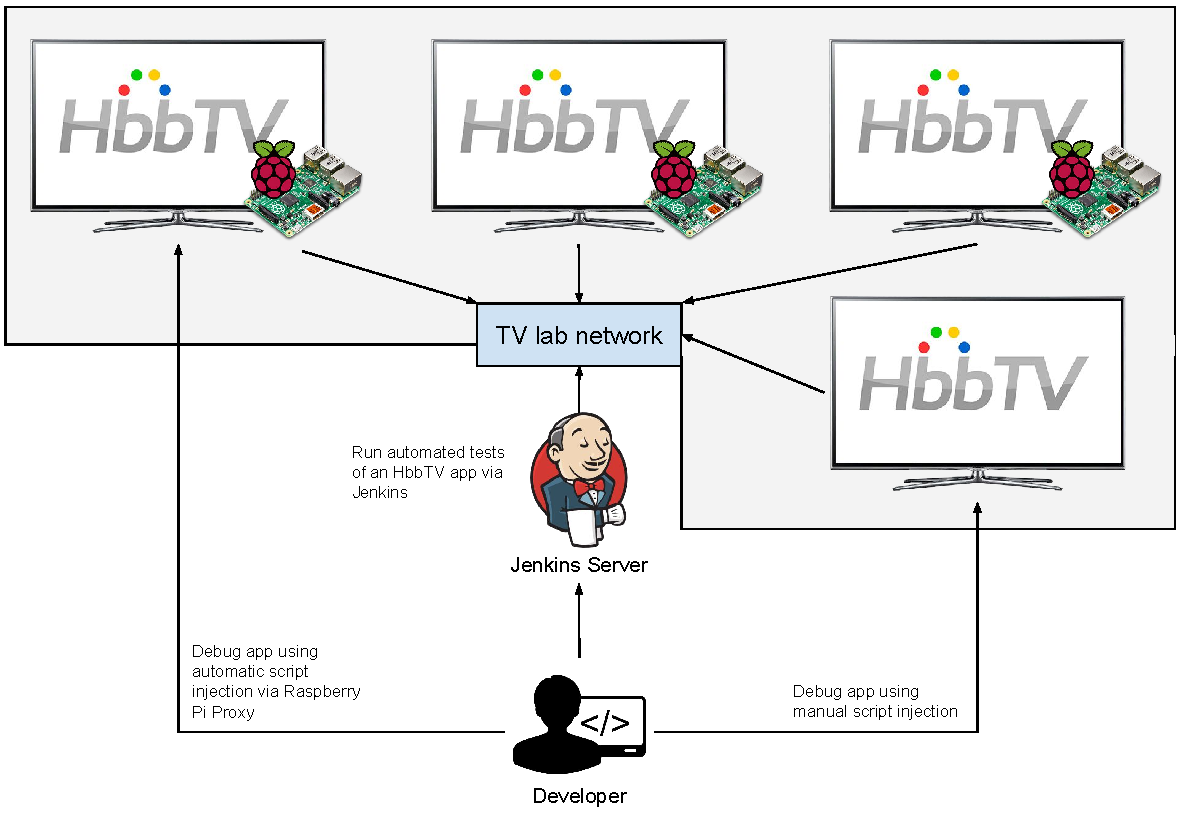
\includegraphics[width=15cm]{big_picture.pdf}\\
  \caption{Big picture of how developers will be able to develop and test their HbbTV application}\label{fig:bigpicture}
\end{figure}

With both platforms in place the developer of an HbbTV app will be able to debug and test his applications
with modern tooling that is used in todays web development. Since the technologies for both is based on
common used and well defined standards we don't restrict ourself to another home grown solution instead we
allow the integration to other tooling which makes us less bound to a certain tool. As described in Figure
\ref{fig:bigpicture} the developer will have three different ways to utilize the TV. One way is to use
a TV that was equipped with a Raspberry Pi running the automation driver on it. The Pi will act as a proxy
and allows to automatically inject the automation script as well as track network data to display it in the
DevTools. Because of the amount of edge cases and issues this proxy can run into there will be no guarantee
that this approach is a bullet proof and easy to use solution. Running this kind of setup requires some amount
of effort to maintain it. That's why there will be another way to debug and test HbbTV apps without a
Raspberry PI. This solution will require some manual changes to the source code of the app to make it work.
To demonstrate the flexibility of the debuging and testing platform I will showcase at the end a common
CI/CD workflow to run automated tests on a real HbbTV app.

\section{Outline\label{sec:outline}}

The 'structure' or 'outline' section gives a brief introduction into the main chapters of
your work. Write 2-5 lines about each chapter. Usually diploma thesis are separated into
6-8 main chapters.\\
\\
\textbf{Chapter \ref{cha:chapter2}} is usually termed 'Related Work', 'State of the Art'
or 'Fundamentals'. Here you will describe relevant technologies and standards related
to your topic. What did other scientists propose regarding your topic? This chapter makes
about 20-30 percent of the complete thesis.\\
\\
\textbf{Chapter \ref{cha:chapter3}} analyzes the requirements for your component. This
chapter will have 5-10 pages.\\
\\
\textbf{Chapter \ref{cha:chapter4}} is usually termed 'Concept', 'Design' or 'Model'.
Here you describe your approach, give a high-level description to the architectural
structure and to the single components that your solution consists of. Use structured
images and UML diagrams for explanation. This chapter will have a volume of 20-30
percent of your thesis.\\
\\
\textbf{Chapter \ref{cha:chapter5}} describes the implementation part of your work. Don't
explain every code detail but emphasize important aspects of your implementation. This
chapter will have a volume of 15-20 percent of your thesis.\\
\\
\textbf{Chapter \ref{cha:chapter6}} is usually termed 'Evaluation' or 'Validation'. How
did you test it? In which environment? How does it scale? Measurements, tests, screenshots.
This chapter will have a volume of 10-15 percent of your thesis.\\
\\
\textbf{Chapter \ref{cha:chapter7}} summarizes the thesis, describes the problems that
occurred and gives an outlook about future work. Should have about 4-6 pages.
